\chapter{Introdução}
\label{cha:introducao}

	O cenário atual de comércio em um mundo intrinsecamente globalizado requer eficiência em troca de informações, serviços e mercadorias; ou seja, eficiência logística. A logística contribui para que pessoas não mais sejam obrigadas a viver perto das fontes de produção e possam trocar informações e mercadorias com outras regiões de forma efetiva, contribuindo decisivamente para melhorar o padrão econômico de vida geral. 
	
	A logística moderna envolve primariamente o compartilhamento de dados. A logística da informação lida com o fluxo de informações entre humanos e/ou máquinas dentro ou entre organizações \cite{haftor2009information}, que se agrupam formando uma rede de criação de valor por meio de informações. 
	
	A Memória Digital do Produto (MDP) é um conceito que se refere a sistemas que permitem a coleta de dados em todas as fases do ciclo de vida do produto para a distribuição e/ou análise. Os dados de interesse do produto podem ser relativos a qualquer fase do produto ao longo de sua cadeia de valor, o que abrange dados de produção individual, de montagem, de distribuição, de uso por parte do consumidor, etc.
	
	A manutenção da MDP permite o compartilhamento de informações do produto ao longo de sua cadeia de suprimentos, fornecendo informações importantes ao fabricante a fim de se aprimorar o desenvolvimento de novas versões do próprio produto. O compartilhamento de informações funciona também como um elo permanente entre o fornecedor e o cliente no pós-venda, permitindo assim que o produto mantenha atualizações de software e quaisquer outras melhorias instantaneamente.
	
	O produto que contém uma memória digital alimentada por meio de sistemas que permitem a coleta de dados em todas as fases do ciclo de vida do produto, pode salvar esse dados e distribuí-los para análise \cite{lasi2014industryfour}. Isso abrange dados de produção, montagem, distribuição (transporte) \cite{brandherm2011productmemory}, padrões de uso pelo cliente final, etc.
	
	Tais dados, aliados a técnicas de Inteligência Empresarial (\textit{Business Intelligence} -- BI) para análise de dados, podem fornecer informações a serem retroalimentadas na fase de desenvolvimento do produto, como forma de identificar pontos de melhorias para o desenvolvimento de novas versões do produto.
	
	Tais conceitos de compartilhamento de informações de produtos por meio da MDP se encaixam na proposta da Indústria 4.0 (I4.0), que tem como fundamentos a inserção de novas tecnologias com o propósito de se oferecer um alto nível de automação e intercâmbio de informações entre equipamentos e produtos \cite{lasi2014industryfour}.
	
	Portanto, surge na I4.0 oportunidades para a criação de novas arquiteturas centradas no amplo compartilhamento de informações ao longo da cadeia de suprimentos, além de novas metodologias para a extração e análise dessas informações para desenvolvimento de outros produtos aperfeiçoados.
	
	A Logística da Informação e, consequentemente, a MDP são intrinsecamente relacionados à I4.0, que por sua vez faz o uso extensivo de conhecimentos e técnicas das área de Gestão da Informação (GI) e Tecnologia de Informação e Comunicação (TIC).
	
	A Indústria 4.0 surgiu a partir da crescente integração das Tecnologias da Informação e Comunicação (TIC) às cadeias de valor industriais, criando as bases para a próxima revolução industrial \cite{hermann2016design}. Essa mudança de paradigma na indústria se refere às recentes modificações em relação às tecnologias de manufatura, que passam a proporcionar um alto nível de automação e intercâmbio de informações entre equipamentos, produtos e demais atores em um ambiente de manufatura \cite{lasi2014industryfour}. 
	
	O nome Indústria 4.0 (I4.0) se dá ao fato de ser considerada a quarta maior revolução com relação à tecnologia de produção industrial, sendo as ``revoluções industriais'' consideradas evoluções tecnológicas que levaram a grandes mudanças no paradigma de produção, tal histórico de revoluções no campo da indústria é ilustrado na \autoref{fig:i4}.
	
	\begin{figure}[htb]
		\centering
		\caption{As revoluções industriais.}
		\label{fig:i4}
		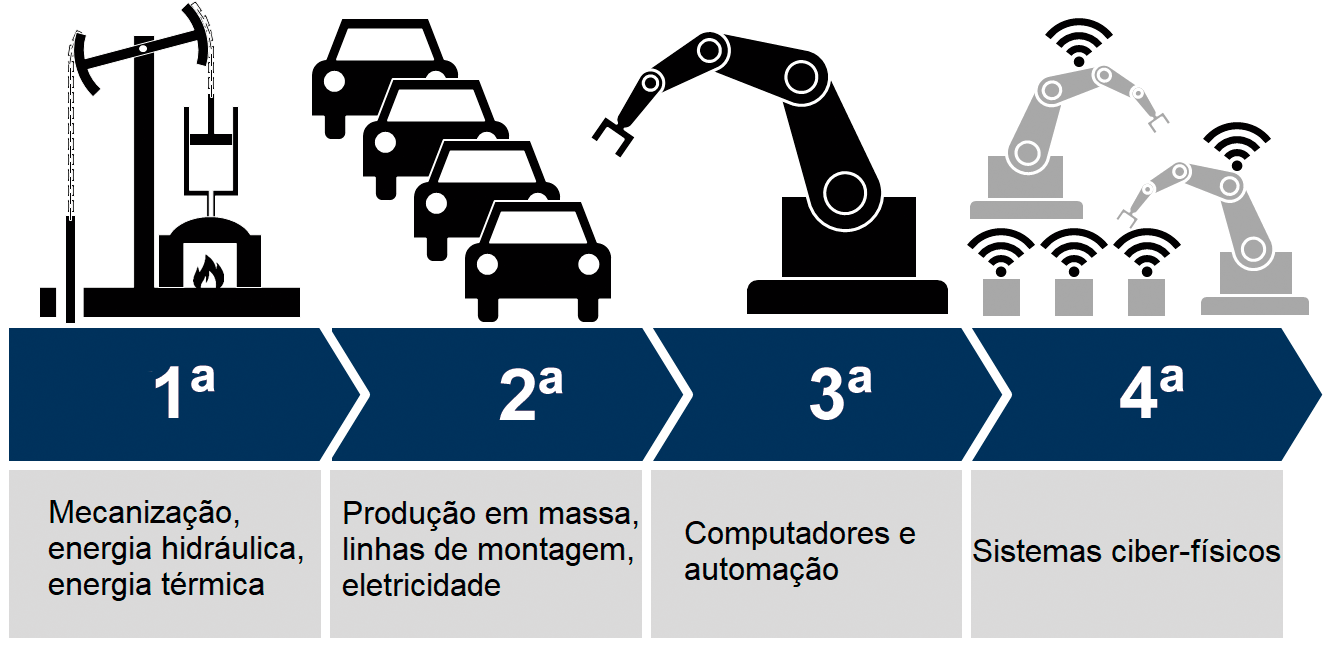
\includegraphics[width=1\textwidth]{i4.png}
		\fonte{\citeonline{lasi2014industryfour} (adaptado).}
	\end{figure}
	
	Tais modificações na indústria são essenciais devido às novas necessidades da própria indústria e de mudança de padrões de consumo do mercado. Isto acarreta mudanças no cenário operacional destas indústrias. Algumas das causas dessas mudanças operacionais são \cite{lasi2014industryfour}:
	
	\begin{itemize}
		
		\item Períodos de desenvolvimento curtos: Os períodos de desenvolvimento e inovação de produtos estão sendo reduzidos. A alta capacidade de inovação está se tornando um fator de sucesso para muitas empresas (\textit{Time to market});
		
		\item Individualização sob demanda: Os compradores passam a definir as condições de compra. Essa tendência leva a uma crescente individualização de produtos com características altamente personalizadas e, em casos extremos, a produtos individuais;
		
		\item Flexibilidade: Devido à individualização sob demanda, novas estruturas e organizações na indústria são essenciais para a fabricação de produtos com alto grau de personalização. É necessária uma maior flexibilidade no desenvolvimento do produto, especialmente na produção;
		
		\item Descentralização: Para lidar com condições específicas de cada produto, são necessários procedimentos mais rápidos de tomada de decisão. Para isso, as hierarquias organizacionais precisam ser reduzidas, dando ao produto maior independência sobre seu próprio processo de fabricação;
		
		\item Eficiência de recursos: A maior eficiência sobre o uso dos recursos sempre é algo desejável, porém sua importância se intensifica com as tendências de aumento dos preços dos recursos, bem como a mudança social no contexto de aspectos ecológicos. Isto exige um foco mais intensivo em sustentabilidade, o que decorre em uma maior racionalidade (ou eficiência) na utilização dos recursos.
		
	\end{itemize}
	
	\citeonline{hermann2016design} elenca alguns princípios para I4.0 que devem ser considerados para o projeto de implementação de soluções I4.0, são eles: Interoperabilidade, transparência de informação, descentralização de decisões e assistência técnica.
	
	Estes princípios são diretrizes para o desenvolvimento de arquiteturas para a I4.0. As arquiteturas surgem com a necessidade de se definir padrões para a implantação de um sistema. Por ser um assunto novo, as arquiteturas de sistemas produtivos voltadas para a quarta revolução industrial também se encontram em estágio inicial \cite{pisching2018arquitetura}. Hoje, o mais consolidado modelo de arquitetura para a Indústria 4.0 é o RAMI4.0 (Modelo de Arquitetura de Referência para a Indústria 4.0). Esse modelo de arquitetura foi apresentado na feira industrial de Hanôver na Alemanha em abril de 2015.
	
	O RAMI4.0 requer uma representação tridimensional, conforme a \autoref{fig:rami4}. Nos três eixos do RAMI4.0 são descritos os níveis hierárquicos de uma fábrica ligada em rede através da Internet (Eixo Níveis Hierárquicos), a representação de arquitetura dos componentes I4.0 (Eixo Camadas) e o ciclo de vida de instalações e de produtos (Eixo Ciclo de Vida e Cadeia de Valor).
	
	\begin{figure}[htb]
		\centering
		\caption{Representação do RAMI4.0.}
		\label{fig:rami4}
		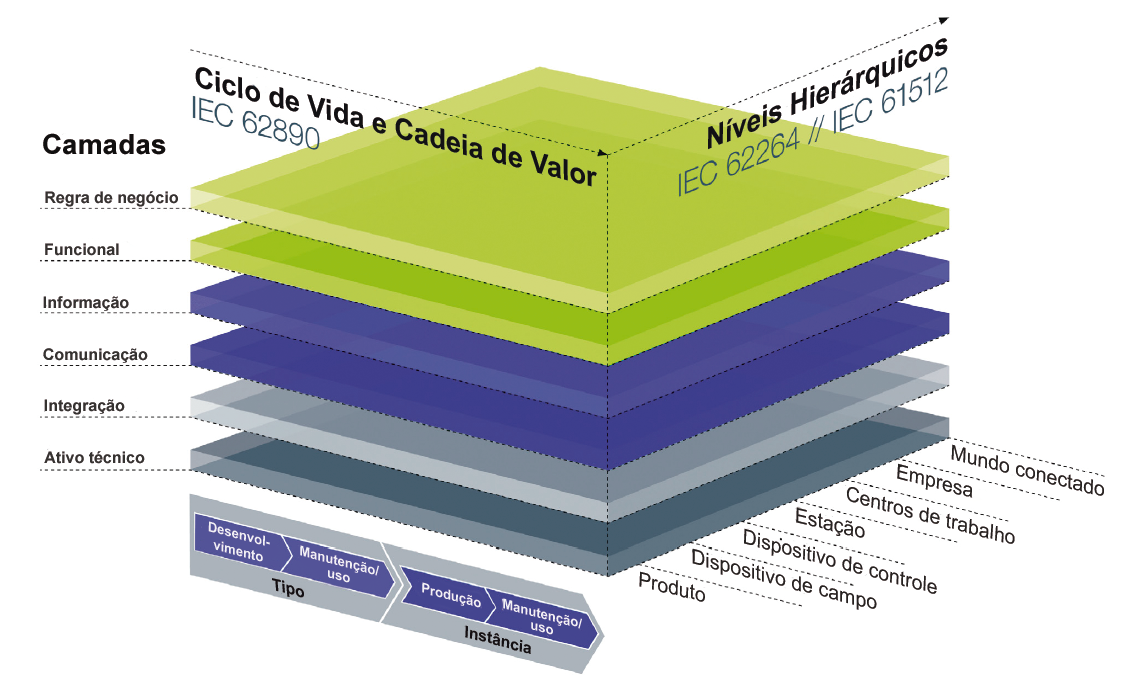
\includegraphics[width=1\textwidth]{rami4.png}
		\fonte{\citeonline{adolphs2015rami} (adaptado).}
	\end{figure}
	
	O RAMI4.0, como um modelo de referência, é um elemento para padronização do projeto e implantação de aplicações em I4.0. O RAMI4.0 é uma padronização de linguagem e deve ser aceito e usados por todos os participantes para protótipo, desenvolvimento e validação.
	
\section{Integração da MDP ao RAMI4.0}

	Ambos os conceitos de I4.0 e MDP são conceitos recentes, surgidos em 2011 \cite{kagermann2011industrie} e 2007 \cite{wahlster2007digitalmemory}, respectivamente . A área multidisciplinar de estudo envolvendo MDP e I4.0 surgira em 2013 com o projeto SemProM \cite{wahlster2013semprom}, porém ainda quando I4.0 era um conceito abrangente e sem diretrizes concretas para sua implementação, que ocorreria em 2013 por meio do documento de recomendações para implementação da iniciativa estratégia Industrie 4.0 \cite{kagermann2013recommendations}; e sem a criação do modelo de arquitetura de referência para Indústria 4.0 (RAMI4.0), que seria divulgada em 2015 por meio do documento entitulado ``RAMI4.0'', divulgado por um periódico alemão \cite{hankel2015rami}.

	Alguns outros estudos como \citeonline{lasi2014industryfour} citam MDP como oportunidade de estudo e aplicação dentro da I4.0, outros como \citeonline{weyer2015standardization} e \citeonline{paelke2014augmented} implementam sistemas práticos envolvendo ambos os conceitos, porém sem considerações sobre cadeia de valor.

	Há estudos na área multidisciplinar de I4.0 e MDP, principalmente no meio acadêmico, empresarial e governamental alemão pelo fato de esses conceitos terem surgido na Alemanha. Porém nenhum trabalho até o presente momento relaciona o modelo de arquitetura de referência para a I4.0 (RAMI4.0) com a MDP. I4.0 e a MDP são conceitos altamente correlacionados, porém ainda não amplamente abordados em conjunto na literatura, o que aponta uma lacuna de conhecimento dentro de I4.0 a ser explorada.

	Estudos sobre o RAMI4.0 são importantes no sentido de padronizar a implementação da I4.0 em empresas de diferentes negócios, garantindo assim a interoperabilidade dos serviços. O eixo ``Ciclo de Vida e Cadeia de Valor'' apresenta diretrizes para o correto planejamento da vida de um produto e sugere cenários para criação de valor perceptível ao produto/serviço. Integrar o conceito de MDP ao RAMI4.0, especificamente ao eixo de ``Ciclo de Vida e Cadeia de Valor'', enriquece o nível de discussão sobre essa arquitetura de referência e dá mais robustez ao modelo para uma futura adoção generalizada por parte de empresas por todo o mundo.

	A ``Plattform Industrie 4.0'' é uma das principais redes mundiais de discussão sobre I4.0 \cite{kagermann2013recommendations, acatech2014plattform, germany2019plattform}. O Conselho de Pesquisa da Plattform Industrie 4.0 é o comitê consultivo estratégico da Plattform Industrie 4.0 e identifica necessidades de pesquisa e ações em torno da I4.0. O comitê identificou e definiu quatro temas-chave de abordagens no setor tecnológico, econômico, metodológico e social/legal para se implementar com sucesso a I4.0 \cite{hirsch-kreinsen2019keythemes}, conforme mostrado na \autoref{fig:keythemes-i4}. Isso significa que os tópicos elencados são temas com alto potencial para a otimização de rotinas e processos de produção existentes no cenário de I4.0.
	
	\begin{figure}[htb]
		\centering
		\caption{Temas-chave de pesquisa e desenvolvimento em I4.0.}
		\label{fig:keythemes-i4}
		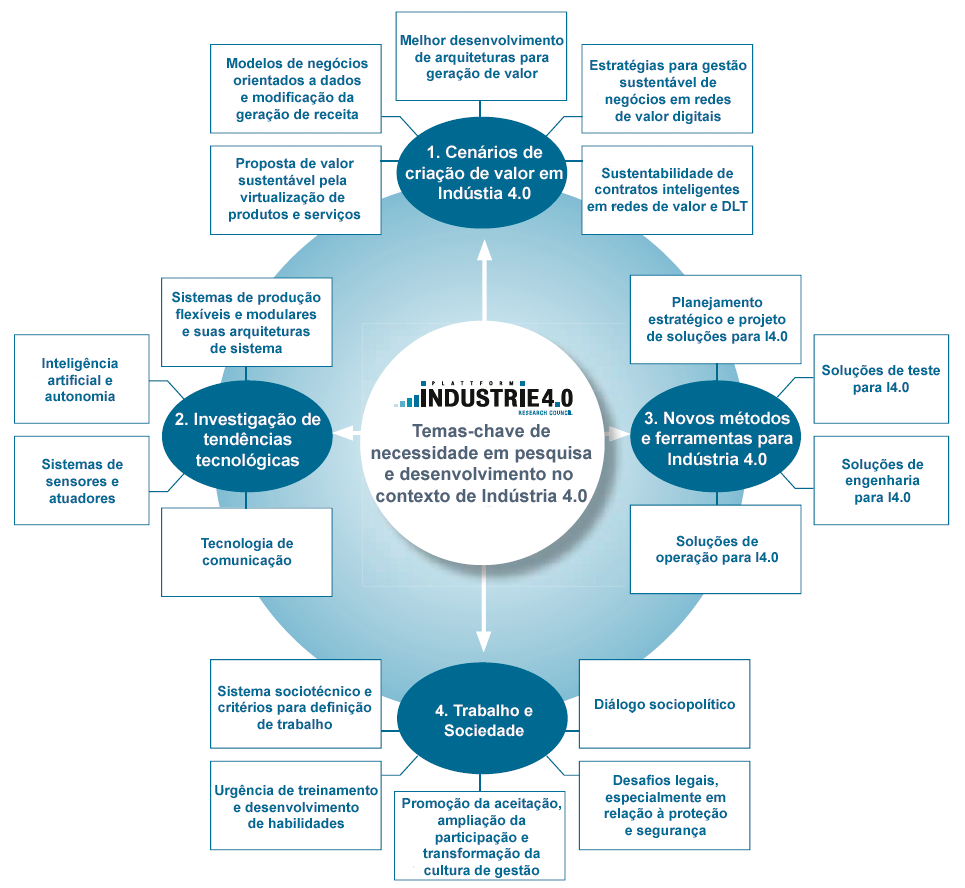
\includegraphics[width=1\textwidth]{keythemes-i4.png}
		\fonte{\citeonline{hirsch-kreinsen2019keythemes} (adaptado).}
	\end{figure}
	
	Dentre os temas elencados na \autoref{fig:keythemes-i4}, destacam-se os subitens relacionados ao tópico ``Cenários de criação de valor em Indústria 4.0'' por estarem altamente relacionados ao RAMI4.0 e ao conceito de geração de valor por meio da MDP. O desenvolvimento de arquiteturas para geração de valor e a criação de negócios orientados a dados são temas de grande oportunidade dentro do cenário de I4.0, especialmente se considerando os métodos quantitativos de \textit{Business Intelligence} e de análise de dados já estabelecidos.

\section{Objetivos}

	O objetivo do trabalho é a proposta de um arquitetura orientada a serviços baseada no RAMI4.0 para o compartilhamento da memória digital do produto ao longo da cadeia suprimentos.
	
	Para isso, é feita uma integração do conceito de MDP ao RAMI4.0, mapeando suas funções ao eixos de Camadas do RAMI4.0.
	
	São feitas também considerações sobre o impacto do amplo compartilhamento da memória digital do produto ao longo da cadeia de suprimentos no ciclo de vida do produto e como isto pode gerar novos modelos de negócio.
	
	Portanto, os eixos ``Camadas'' e ``Ciclo de Vida e Cadeia de Valor'' são detalhados, de forma a se aperfeiçoar a elaboração dessa arquitetura a fim de proporcionar mais robustez ao modelo para uma futura adoção generalizada por parte de empresas por todo o mundo.
	
	Todo o estudo é feito com a proposta de aperfeiçoar o RAMI4.0 no sentido de propiciar o surgimento de novos cenários de criação de valor no contexto de I4.0 e incentivar geração de novos modelos de negócio, especialmente aqueles baseados em dados (\textit{data-driven}).
		
	Esta pesquisa envolve o estudo de diversos temas relacionados à Indústria 4.0. Os principais itens necessários para a elaboração da arquitetura de compartilhamento de dados são fundamentados no \autoref{cha:fundamentos}.
	
	Tais temas são estudados a fim de se analisar o estado da arte atual em I4.0 e a partir disso propor melhorias e detalhamentos ao RAMI4.0.

\section{Estrutura do trabalho}

	
	O capítulo atual de introdução (\autoref{cha:introducao}) apresenta uma abordagem inicial aos conceitos que serão tratados ao longo do trabalho e o objetivo da pesquisa.
	
	O \autoref{cha:metodologia} detalha a metodologia de pesquisa adotada ao longo do todo o projeto de pesquisa.
	
	O \autoref{cha:fundamentos} mostra a revisão bibliográfica realizada para a fundamentação dos conceitos necessários para a proposta da arquitetura de compartilhamento de informações do ativo. Cinco conceitos básicos são apresentados nesse capítulo: ``Indústria 4.0'', ``Logística \& Cadeia de Suprimentos'', ``Ciclo de vida do produto'', ``Memória digital do produto'' e ``Arquitetura orientada a serviços''.
	
	O \autoref{cha:arquitetura} apresenta os detalhes da arquitetura proposta baseada em \textit{Web Services} (WS) nos modelos de uma arquitetura orientada a serviços (SOA) compatível com Componentes I4.0 para o compartilhamento de informações do ativo ao longo da cadeia de suprimentos. Neste capítulo também é feito o mapeamento dos componentes desta arquitetura a cada um dos níveis do eixo Camadas do RAMI4.0.
	
	O \autoref{cha:ciclo-de-vida} traz discussões sobre o impacto do amplo compartilhamento da memória digital do produto ao longo da cadeia de suprimentos por meio de \textit{Web Services}, são abordadas possíveis mudanças na curva de ciclo de vida do produto e o surgimento de novos modelos de negócio baseado em dados.
	
	O \autoref{cha:prova-de-conceito} detalha uma possível implementação da arquitetura proposta utilizando algumas tecnologias atualmente consolidadas na área de \textit{Engenharia de Software}.
	
	Finalmente, no \autoref{cha:conclusao} são feitas as considerações finais sobre a pesquisa e uma conclusão sobre os resultados alcançados.
	
	